% !TEX root=../../mt-motion-analysis.tex
\chapter{Introduction}
Among the physically active young to middle aged population injuries to e.g. knee or hip are common. In a study by Thorborg et al. 49\% of the questioned sub-elite football players in Denmark reported they had issues with hip and/or groin pain during the previous season \cite{Thorborg2017}. Among serious injuries rupture of the \gls{acl} is one of the more severe and common. Moses et al. show annual \gls{acl} injury incidence rates of up to 1.62\% for amateur athletes \cite{Moses2012}. Treatment of such injuries is a debated subject and whether surgery yields better results is difficult to say \cite{Krause2018, Monk2016}. Independently of the treatment the patient needs to undergo a long rehabilitation process.
Apart from the rehabilitation an injury may also lead to long term physical impairments, such as joint instability \cite{Ageberg2002} and increased risk of knee ostearthritis (OA) \cite{Lohmander2007}, as well as increased risk of depression \cite{Crichlow2006} and re-injury \cite{Paterno2012}.

The \gls{acl} can be seen in Figure \ref{fig:acl} and is one of the ligaments connecting the femur (thigh bone) with the tibia (shin bone) and is one of the key structures for providing stability in the knee \cite{Duthon2006}. Injuries to the \gls{acl} commonly occurs without any direct contact from e.g. other athletes. Instead a typical injury mechanism is a sudden change of direction or velocity while the knee bears weight \cite{Wetters2016}.

\begin{figure}
  \centering
  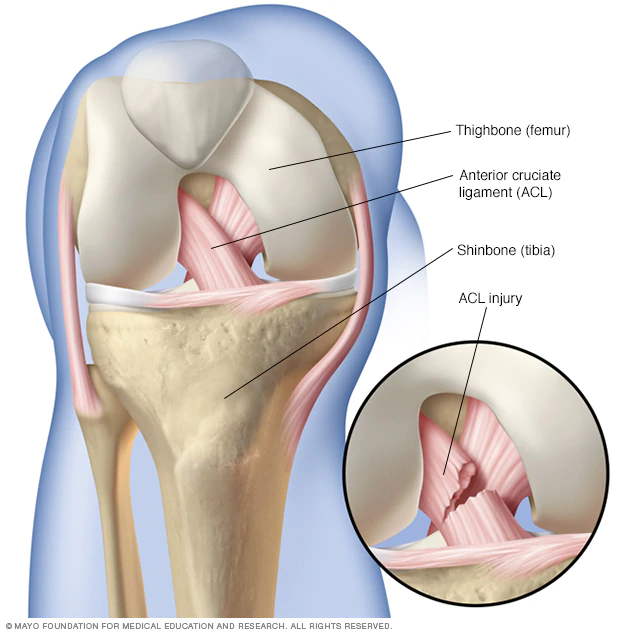
\includegraphics[width=0.5\textwidth]{files/figs/acl.png}
  % \caption{Illustration of the position of the ACL in the knee and a ruptured ACL. Image from \cite{MayoACL}.}
  \caption{Illustration of the position of the ACL in the knee. Image from \cite{MayoACL}.}
  \label{fig:acl}
\end{figure}

% \section{ACL anatomy}

\section{Postural Orientation Errors}
The ability to uphold the alignment of body segments, both in relation to each other and the surroundings, is called postural orientation \cite{Horak2006}. Altered postural orientation, or \glspl{poe}, has been seen to increase the risk of suffering new injuries \cite{Hewett2005}, hence this is an important measure during rehabilitation and before return to sports. 3D motion capture systems are considered to be the "gold standard" for measurement of postural orientation. This is, however, an expensive and time consuming procedure, requiring specific resource in terms of laboratories and experts to perform the measurements. A potential alternative, more suitable for clinical use, is visual assessments of 2D measurements (i.e. videos) \cite{Nae2020}.

There is not one established method for visual assessments of postural orientation errors, but Nae et al. presented a test battery where up to six segment specific \glspl{poe} were assessed for five different functional tasks. Each \gls{poe} was scored on an ordinal scale from 0 to 2 \cite{Nae2017, Nae2020b}. A detailed explanation of the \gls{poe}-task combinations can be found in Appendix \ref{app:poe-task}. This scoring system is the foundation of this thesis, but in this work we only study the femoral valgus-, deviation of trunk-, deviation of pelvis-, and knee medial to foot position-\glspl{poe} for the single leg squat task. The evaluated \glspl{poe} and task are described in Section \ref{ngnstans..} (SKA DETTA BESKRIVAS H'R? ELLER EN EGEN SECTION? ELLER I METHOD?)


% \begin{table}
%  \centering
%  \caption{Motion-POE combinations available in the data.}
%  \label{tab:met:motion-poes}
%
%  \begin{tabular}{|c|ccccc|}
%   \hline
%   \backslashbox{POE}{Motion}                      &
%   \multicolumn{1}{c}{\begin{tabular}[c]{@{}c@{}}Single\\ leg squat\end{tabular}}   &
%   \multicolumn{1}{c}{\begin{tabular}[c]{@{}c@{}}Stair\\ descending\end{tabular}}   &
%   \multicolumn{1}{c}{\begin{tabular}[c]{@{}c@{}}Forward\\ lunge\end{tabular}}   &
%   \multicolumn{1}{c}{\begin{tabular}[c]{@{}c@{}}Single leg hop\\ for distance\end{tabular}}   &
%   \multicolumn{1}{c|}{\begin{tabular}[c]{@{}c@{}}Side\\ hop\end{tabular}}                      \\ \hline \hline
%
%   \multicolumn{1}{|c|}{\begin{tabular}[c]{@{}c@{}}Deviation of trunk\\ in any plane\end{tabular}}                 & x & x &   & x & x \\ \hdashline
%   \multicolumn{1}{|c|}{\begin{tabular}[c]{@{}c@{}}Deviation of pelvis\\ in any plane\end{tabular}}                & x & x & x & x & x \\ \hdashline
%   \multicolumn{1}{|c|}{\begin{tabular}[c]{@{}c@{}}Femoral\\ valgus\end{tabular}} &
%   x                                               & x & x & x & x     \\ \hdashline
%   \multicolumn{1}{|c|}{\begin{tabular}[c]{@{}c@{}}Knee medial to\\ foot position\end{tabular}} &
%   x                                               & x & x & x & x     \\ \hdashline
%   \multicolumn{1}{|c|}{\begin{tabular}[c]{@{}c@{}}Femur medial\\ to shank\end{tabular}} &
%   x                                               & x & x & x & x     \\ \hdashline
%   \multicolumn{1}{|c|}{\begin{tabular}[c]{@{}c@{}}Foot\\ pronation\end{tabular}}                                           & x &   &   &   &   \\ \hline
%  \end{tabular}
% \end{table}


\section{Related / Previous work (typ kombination medicin/ml)}
https://ieeexplore.ieee.org/document/7592162 lol
https://pubmed.ncbi.nlm.nih.gov/29204327/ lololol
https://www.sciencedirect.com/science/article/pii/S2468781218301590?via%3Dihub

\section{avgr'nsningar eller typ m]l med detta arbete}
typ om att bara SLS analyseras? och lite s[nt.. kanske att 3d inte utv'rderas? eller att det utv'rderades litgrann??

skriv om att detta 'r ett proof of concept, att bara sls analyseras osv

sen typ report outline


introducera poe  (skriv mer om det i section)

skriv om risker med bias fr dataset osv... kansek ska n'mnas i dl-kapitlet?


% @article{Monk2016,
% author = {Monk, AP, Davies, LJ, Hopewell, S, Harris, K, Beard, DJ, and Price, AJ},
% title = {Surgical versus conservative interventions for treating anterior cruciate ligament injuries},
% journal = {Cochrane Database of Systematic Reviews},
% number = {4},
% year = {2016},
% publisher = {John Wiley & Sons, Ltd},
% ISSN = {1465-1858},
% DOI = {10.1002/14651858.CD011166.pub2},
% keywords = {*Anterior Cruciate Ligament Injuries; Adult; Anterior Cruciate Ligament Reconstruction [*methods]; Humans; Joint Instability [etiology, rehabilitation, *therapy]; Randomized Controlled Trials as Topic; Young Adult},
% URL = {https://doi.org//10.1002/14651858.CD011166.pub2}
% }
